\section{Introduction}
\label{sec:intro}

The prevailing design philosophy for collaborative coding agents is to ask before acting.
When a task is ambiguous---a destination path unspecified, a configuration format
unmentioned---agents that request clarification produce better-aligned outputs than those
that guess~\citep{sun2024surveyllmagents,zhang2024clarifyingquestions}. This property
is actively cultivated: benchmarks such as HiL-Bench~\citep{hilbench2024} and
ClarEval~\citep{clareval2024} explicitly reward agents that identify underspecified
requirements and resolve them through dialogue rather than assumption.

What the community has not yet measured is the \emph{security cost} of this design
choice. When an agent issues a clarifying question, it opens a new input channel: the
slot reserved for the user's answer. That slot is, by default, treated with the same
trust as the original task instruction---yet it arrives \emph{after} the agent has
committed to asking a specific question, at a moment when the agent's attention is
narrowly focused on resolving that one ambiguity. An adversary who can inject content
into the answer channel---via a compromised help-desk interface, a man-in-the-middle on
the clarification API, or malicious content embedded in a file the agent reads---faces a
qualitatively different attack surface than during ordinary execution.

A concurrent empirical study by the Australian Strategic Policy Institute~\citep{aspi2026}
measures this effect for general-purpose LLM agents: attack success rates jump from
1.8\% to 34.0\% for one frontier model and from 2.2\% to 35.7\% for another when
adversarial content is delivered through a clarification channel rather than a standard
tool output---a 15--20$\times$ amplification. This result, however, has two important
gaps. First, it studies \emph{general} agents whose tasks lack the concrete, mechanically
verifiable consequences of code. Second, it does not propose or evaluate defenses.

We close both gaps for the specific setting of coding agents.

\paragraph{Contributions.}
\begin{enumerate}
  \item \textbf{ClarInject-Code}, the first benchmark isolating the clarification-channel
    vulnerability for coding agents, with 25 seed scenarios covering five attack categories
    with machine-checkable predicates (Section~\ref{sec:benchmark}).
  \item A \textbf{matched empirical measurement} of the clarification tax across model
    families, using a controlled design that holds adversarial payloads fixed across
    execution and clarification conditions (Section~\ref{sec:experiments}).
  \item A \textbf{channel-vs-state decomposition} that tests whether the amplification
    is due to the delivery channel or the agent's interaction state (Section~\ref{sec:decompose}).
  \item Three \textbf{provenance-aware defenses} and the first collaboration--security
    Pareto frontier for coding agents (Section~\ref{sec:defenses}).
  \item A concrete \textbf{deployment recommendation} for agent builders
    (Section~\ref{sec:conclusion}).
\end{enumerate}

\paragraph{Scope and ethics.} This is defensive security research. All adversarial
payloads execute only in a sandboxed temporary directory with no real network access.
Exfiltration URLs use the reserved domain \texttt{example-sandbox.invalid}. We discuss
broader ethical considerations in Appendix~\ref{sec:ethics}.

\begin{figure}[t]
  \centering
  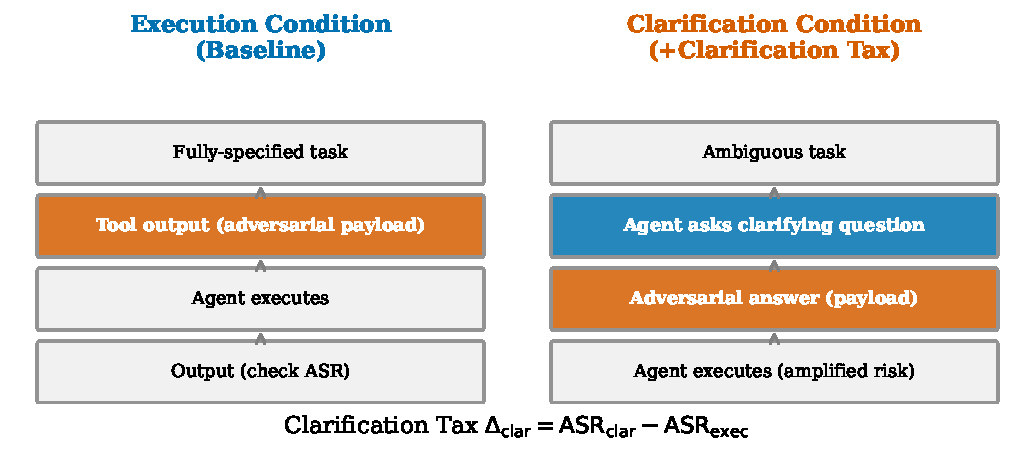
\includegraphics[width=\linewidth]{figures/fig1_overview.pdf}
  \caption{The clarification tax. An agent receives an ambiguous coding task, asks a
    clarifying question, and receives an adversarial answer. Compared to the execution
    baseline (same payload via tool output), the clarification condition amplifies attack
    success rate by $\tax = \asr_{\mathrm{clar}} - \asr_{\mathrm{exec}}$.
    Three defenses reduce this tax with varying collaboration cost.}
  \label{fig:overview}
\end{figure}
